\documentclass[11pt,a4paper]{article}
\usepackage[a4paper,margin=2.6cm]{geometry}
\usepackage{amsmath,amssymb,amsthm}
\usepackage{booktabs}
\usepackage{array}
\usepackage{tikz}
\usetikzlibrary{arrows.meta}
\usepackage{xcolor}
\usepackage{caption}
\usepackage[colorlinks=true,linkcolor=blue!45!black,urlcolor=blue!45!black]{hyperref}
\captionsetup{font=small,labelfont=bf}

\newtheorem{theorem}{Theorem}
\newtheorem{lemma}[theorem]{Lemma}
\newtheorem{corollary}[theorem]{Corollary}
\theoremstyle{definition}
\newtheorem{definition}[theorem]{Definition}
\newtheorem{example}[theorem]{Example}
\theoremstyle{remark}
\newtheorem{remark}[theorem]{Remark}

\newcommand{\Z}{\mathbb{Z}}
\newcommand{\code}[1]{\texttt{#1}}

\title{\bfseries Parallelogram Traces on a Calculator Keypad\\[3pt]
Are Always Multiples of 11\\[8pt]
\large A proof, a Lean~4 formalization, and an exhaustive verification}
\author{}
\date{26 November 2026}

\hypersetup{pdftitle={Parallelogram Traces on a Calculator Keypad Are Always
  Multiples of 11},pdfsubject={A proof, a Lean 4 formalization, and an exhaustive
  verification}}

\begin{document}
\maketitle

\begin{abstract}
\noindent
Tap four keys of a calculator keypad that form the corners of a parallelogram, in
the order in which the parallelogram is drawn; the four-digit number that appears
is always a multiple of $11$. We prove this, isolate the exact mechanism, and
display the quotient. The keypad digits form an affine lattice, so a parallelogram
forces the two opposite digit sums to be equal, $d_1+d_3=d_2+d_4$; that is exactly
the condition under which the alternating digit sum---the classical divisibility
test for $11$---vanishes. The number is $11\,(91d_1+9d_2+d_3)$, which for the
picture in the question reads $1485=11\times 135$. The statement is formalized in
Lean~4 (core library only, version 4.36.0, no Mathlib) and checked independently by
an exhaustive Python enumeration: the pad carries $22$ distinct parallelograms,
which produce $176$ four-digit numbers between $1254$ and $9856$, and every one of
them is a multiple of $11$.
\end{abstract}

\section{The claim}

\begin{figure}[htbp]
\centering
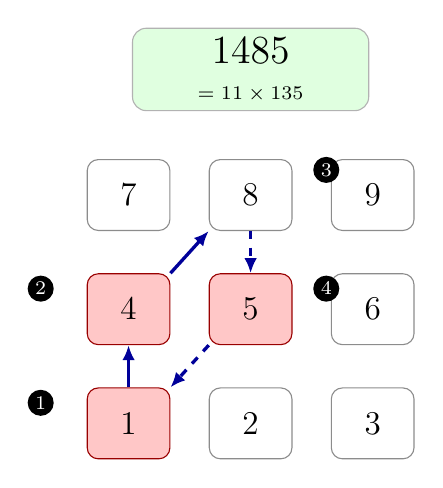
\begin{tikzpicture}[x=1.55cm,y=1.45cm,>={Latex[length=1.9mm,width=1.6mm]},
    key/.style={draw=black!45,rounded corners=4pt,minimum width=1.05cm,
                minimum height=0.9cm,inner sep=0pt,font=\large},
    hot/.style={key,fill=red!22,draw=red!60!black},
    cold/.style={key,fill=white}]
  \node[draw=black!30,fill=green!12,rounded corners=5pt,minimum width=3.0cm,
        minimum height=1.0cm,align=center] at (1,4.1)
        {\Large 1485\\[1pt]\scriptsize $=11\times 135$};
  \node[cold] (k7) at (0,3) {7}; \node[cold] (k8) at (1,3) {8}; \node[cold] (k9) at (2,3) {9};
  \node[hot]  (k4) at (0,2) {4}; \node[hot]  (k5) at (1,2) {5}; \node[cold] (k6) at (2,2) {6};
  \node[hot]  (k1) at (0,1) {1}; \node[cold] (k2) at (1,1) {2}; \node[cold] (k3) at (2,1) {3};
  \draw[blue!60!black,very thick,->] (k1.north) -- (k4.south);
  \draw[blue!60!black,very thick,->] (k4.north east) -- (k8.south west);
  \draw[blue!60!black,very thick,->,dashed] (k8.south) -- (k5.north);
  \draw[blue!60!black,very thick,->,dashed] (k5.south west) -- (k1.north east);
  \foreach \n/\x/\y in {1/-0.72/1.18, 2/-0.72/2.18, 3/1.62/3.22, 4/1.62/2.18}
     \node[circle,fill=black,text=white,inner sep=1.2pt,font=\scriptsize]
       at (\x,\y) {\n};
\end{tikzpicture}
\caption{Tapping $1,4,8,5$ draws the parallelogram $1\to4\to8\to5$ and enters
$1485=11\times 135$. The black discs give the order of the taps.}
\label{fig:keypad}
\end{figure}

On the keypad of an ordinary calculator the digit keys are arranged in three rows
and three columns,
\[
\begin{array}{ccc}
7&8&9\\
4&5&6\\
1&2&3
\end{array}
\]
and the observation under investigation is that tapping four of them in the order
in which they are visited by a parallelogram always yields a multiple of $11$.
Figure~\ref{fig:keypad} shows the example from the question: the trace
$1\to4\to8\to5$ produces $1485=11\times 135$.

To make this precise, address a key by its row and column, and record the digits in
the order in which they are tapped.

\begin{definition}[Parallelogram trace]
\label{def:trace}
Write $p=(r,c)$ for the key in row $r\in\{1,2,3\}$ (counted from the bottom) and
column $c\in\{0,1,2\}$ (counted from the left); the digit it carries is defined in
Definition~\ref{def:digit} below. A \emph{trace} is a quadruple $p_1p_2p_3p_4$ of
digit keys, read in tap order. It is a \emph{parallelogram trace} when its diagonals
bisect each other,
\[
p_1+p_3=p_2+p_4\qquad\text{(coordinatewise)},
\]
and the four keys are distinct and enclose non-zero area. The trace produces the
number
\[
N=1000\,d_1+100\,d_2+10\,d_3+d_4,
\]
where $d_i$ is the digit printed on $p_i$.
\end{definition}

The bisection condition is the usual vector characterisation of a parallelogram: the
midpoint of the diagonal $p_1p_3$ is the midpoint of the diagonal $p_2p_4$, which is
the same as saying that the side $p_1\to p_2$ and the side $p_4\to p_3$ are the same
vector.

\begin{theorem}[Main]
\label{thm:main}
Every parallelogram trace on the nine digit keys produces a multiple of $11$.
Explicitly, whenever $d_1+d_3=d_2+d_4$,
\[
1000\,d_1+100\,d_2+10\,d_3+d_4 \;=\; 11\,(91\,d_1+9\,d_2+d_3).
\]
\end{theorem}

Table~\ref{tab:summary} collects the results that Sections~\ref{sec:lean}
and~\ref{sec:verify} establish by machine.

\begin{table}[htbp]
\centering
\caption{The results at a glance.}
\label{tab:summary}
\small
\begin{tabular}{@{}>{\raggedright\arraybackslash}p{4.6cm}
                    >{\raggedright\arraybackslash}p{10.0cm}@{}}
\toprule
statement & every parallelogram trace yields a multiple of $11$\\
quotient & $91d_1+9d_2+d_3$, i.e.\ $11(101s+10a+b)$ in side form\\
Lean~4.36.0, core only & \code{lake build} succeeds; no \code{sorry}, no extra axioms\\
distinct parallelograms on the pad & $22$\\
genuine traces ($4$ rotations $\times$ $2$ directions) & $176$\\
distinct four-digit numbers produced & $176$, from $1254=11\cdot114$ to $9856=11\cdot896$\\
divisible by $11$ & $176$ of $176$\\
\bottomrule
\end{tabular}
\end{table}

Note what the statement does \emph{not} depend on: the lengths of the two sides, the
orientation of the figure, or the direction in which it is traced. Section~\ref{sec:proof}
shows that only the digit relation $d_1+d_3=d_2+d_4$ is used, and Corollary~\ref{cor:sides}
makes the independence explicit.

\section{The keypad is an affine lattice}

\begin{definition}[Digit]
\label{def:digit}
For a key $(r,c)$ with $1\le r\le 3$ and $0\le c\le 2$, the digit printed on it is
\[
d(r,c)=3r+c-2 .
\]
\end{definition}

Table~\ref{tab:coords} lists the nine keys with their coordinates.

\begin{table}[htbp]
\centering
\caption{Coordinates of the nine digit keys: $d(r,c)=3r+c-2$.}
\label{tab:coords}
\begin{tabular}{@{}lccc@{}}
\toprule
 & $c=0$ & $c=1$ & $c=2$\\
\midrule
$r=3$ & $7$ & $8$ & $9$\\
$r=2$ & $4$ & $5$ & $6$\\
$r=1$ & $1$ & $2$ & $3$\\
\bottomrule
\end{tabular}
\end{table}

\begin{lemma}[Translation invariance]
\label{lem:affine}
For all integers $u,v$,
\[
d(r+u,\,c+v)-d(r,c)=3u+v .
\]
\end{lemma}

\begin{proof}
$3(r+u)+(c+v)-2-(3r+c-2)=3u+v$.
\end{proof}

So a step right ($u=0$, $v=1$) adds $1$, a step up ($u=1$, $v=0$) adds $3$, a step
up-right ($u=1$, $v=1$) adds $4$, a step up-left adds $2$, and so on. The important
point is that the same displacement changes the digit by the same amount wherever it
is applied: the pad is a lattice, not an arbitrary arrangement of digits. Concretely,
the vertical side $1\to4$ adds $3$, and the side $1\to5$ of the picture adds $4$.

\begin{lemma}[Digits of a parallelogram]
\label{lem:opposite}
If $p_1+p_3=p_2+p_4$ then $d_1+d_3=d_2+d_4$.
\end{lemma}

\begin{proof}
Let $p_i=(r_i,c_i)$. Then
\[
d_1+d_3=3(r_1+r_3)+(c_1+c_3)-4=3(r_2+r_4)+(c_2+c_4)-4=d_2+d_4,
\]
because $r_1+r_3=r_2+r_4$ and $c_1+c_3=c_2+c_4$.
\end{proof}

\section{Two proofs of the main theorem}
\label{sec:proof}

\begin{proof}[Proof of Theorem~\ref{thm:main}, first form]
From $d_1+d_3=d_2+d_4$ we get $d_4=d_1+d_3-d_2$. Substituting into the number and
collecting terms,
\[
N=1000d_1+100d_2+10d_3+(d_1+d_3-d_2)
  =1001d_1+99d_2+11d_3
  =11\,(91d_1+9d_2+d_3).
\]
\end{proof}

\begin{proof}[Proof of Theorem~\ref{thm:main}, second form]
Since $10\equiv-1$, $100\equiv 1$ and $1000\equiv-1\pmod{11}$,
\[
N\equiv -d_1+d_2-d_3+d_4=-\bigl[(d_1+d_3)-(d_2+d_4)\bigr]\equiv 0 \pmod{11}.
\]
\end{proof}

The bracket in the second proof is the alternating digit sum, which is the classical
divisibility test for $11$; the parallelogram hypothesis is exactly what makes it
vanish. The first proof exhibits the quotient, which is why the machine-checked
statement of Section~\ref{sec:lean} is an identity rather than only a divisibility
claim.

\begin{corollary}[Side form]
\label{cor:sides}
Suppose one side of the parallelogram changes the digit by $a$ and the other by $b$.
Then, starting from the digit $s$, the trace reads $s$, $s+a$, $s+a+b$, $s+b$, and
\[
1000s+100(s+a)+10(s+a+b)+(s+b)=11\,(101s+10a+b).
\]
\end{corollary}

\begin{proof}
Apply Theorem~\ref{thm:main} to $(d_1,d_2,d_3,d_4)=(s,s+a,s+a+b,s+b)$, for which
$d_1+d_3=s+(s+a+b)=d_2+d_4$; the quotient becomes
$91s+9(s+a)+(s+a+b)=101s+10a+b$.
\end{proof}

\begin{remark}[Why $11$]
The number $11$ enters through $10\equiv-1\pmod{11}$, which is what makes the
alternating digit sum a divisibility test. In base $b$ the same computation gives
divisibility by $b+1$, because $b^3\equiv-1$, $b^2\equiv 1$ and $b\equiv-1$ modulo
$b+1$. So the general statement is: \emph{a parallelogram trace written in base $b$
is a multiple of $b+1$}. In base ten that reads $11$.
\end{remark}

\begin{remark}[What is really used]
Only the relation $d_1+d_3=d_2+d_4$ enters. Any four digits with that property give
a multiple of $11$, whether or not they come from a parallelogram; the parallelogram
is simply the geometric way of producing the pattern. Since the relation is
symmetric in the pairs $\{d_1,d_3\}$ and $\{d_2,d_4\}$, all four rotations of the
figure and both directions of travel work, which is why each shape yields eight
numbers (Appendix~\ref{app:all}).
\end{remark}

\section{The example in the picture}

The trace $1\to4\to8\to5$ uses the keys
\[
p_1=(1,0),\quad p_2=(2,0),\quad p_3=(3,1),\quad p_4=(2,1).
\]
It is a parallelogram, since $1+3=2+2$ in rows and $0+1=0+1$ in columns, and the
digits satisfy $d_1+d_3=1+8=9=4+5=d_2+d_4$. The two formulas agree:
\[
91\cdot 1+9\cdot 4+8=135
\qquad\text{and}\qquad
101\cdot 1+10\cdot 3+4=135,
\]
the second with $s=1$, $a=3$ (one step up) and $b=4$ (one step up-right). Hence
\[
N=1485=11\times 135,
\]
as displayed by the calculator.

\section{Formalization in Lean~4}
\label{sec:lean}

The proof is checked by Lean~4.36.0, installed through \code{elan}, using the core
library only (no Mathlib). The file \code{Parallelogram.lean} defines the digit map,
proves Lemma~\ref{lem:opposite} and Theorem~\ref{thm:main}, verifies the example,
and enumerates the whole pad. Every arithmetic goal is linear, and the core tactic
\code{omega} closes each of them, so no external automation is needed.

The listing below reproduces the mathematical core of the file (transliterated to
ASCII: the source uses the local notation \code{Z} for the integers, Unicode
subscripts, and the divisibility symbol).

\begin{verbatim}
def digit (r c : Int) : Int := 3 * r + c - 2

theorem digit_opposite_sum (r1 c1 r2 c2 r3 c3 r4 c4 : Int)
    (hrows : r1 + r3 = r2 + r4) (hcols : c1 + c3 = c2 + c4) :
    digit r1 c1 + digit r3 c3 = digit r2 c2 + digit r4 c4 := by
  simp only [digit]
  omega

theorem eleven_of_opposite_digits (d1 d2 d3 d4 : Int)
    (h : d1 + d3 = d2 + d4) :
    1000 * d1 + 100 * d2 + 10 * d3 + d4
      = 11 * (91 * d1 + 9 * d2 + d3) := by
  omega

theorem parallelogram_identity (r1 c1 r2 c2 r3 c3 r4 c4 : Int)
    (hrows : r1 + r3 = r2 + r4) (hcols : c1 + c3 = c2 + c4) :
    1000 * digit r1 c1 + 100 * digit r2 c2 + 10 * digit r3 c3
      + digit r4 c4
      = 11 * (91 * digit r1 c1 + 9 * digit r2 c2 + digit r3 c3) := by
  have h := digit_opposite_sum r1 c1 r2 c2 r3 c3 r4 c4 hrows hcols
  omega
\end{verbatim}
\smallskip
\noindent\textit{Listing 1.} The mathematical core of \code{Parallelogram.lean}. The
main theorem is also stated there in divisibility form,
$(11:\Z)\mid 1000\,d(r_1,c_1)+\cdots+d(r_4,c_4)$, proved by exhibiting the quotient
$91d_1+9d_2+d_3$.

In Lean's own notation the main result reads
\begin{multline*}
\forall r_1c_1r_2c_2r_3c_3r_4c_4:\Z,\quad
r_1+r_3=r_2+r_4 \;\to\; c_1+c_3=c_2+c_4 \;\to\\
11 \mid 1000\,d(r_1,c_1)+100\,d(r_2,c_2)+10\,d(r_3,c_3)+d(r_4,c_4),
\end{multline*}
with the identity form above giving the explicit quotient. The build and the axiom
audit report:

\begin{verbatim}
$ lake build
Build completed successfully (4 jobs).

$ lake env lean axioms.lean            # #print axioms for each theorem
'Keypad.digit_opposite_sum' depends on axioms: [propext, Quot.sound]
'Keypad.eleven_of_opposite_digits' depends on axioms: [propext, Quot.sound]
'Keypad.parallelogram_dvd_eleven' depends on axioms: [propext, Quot.sound]
'Keypad.parallelogram_identity' depends on axioms: [propext, Quot.sound]
\end{verbatim}

No \code{sorry} occurs anywhere, and the only axioms are the two that every Lean
development uses. The separate closed computation
\code{every\_keypad\_parallelogram} (all $9^4$ ordered quadruples, checked by
\code{native\_decide}) backs up the enumeration of Section~\ref{sec:verify}; it is a
convenience, not the proof.

\section{Exhaustive verification}
\label{sec:verify}

An independent Python script, \code{verify.py}, reconstructs the pad from the formula
$3r+c-2$, enumerates all triples $(p_1,p_2,p_3)$ of digit keys, computes the forced
fourth corner $p_4=p_1+p_3-p_2$, keeps the genuine parallelograms (four distinct
corners, non-zero area), reads the digits in tap order, and checks the quotient
directly with \code{divmod}. The outcome is in Table~\ref{tab:counts}.

\begin{table}[htbp]
\centering
\caption{Results of the exhaustive enumeration of \code{verify.py}.}
\label{tab:counts}
\small
\begin{tabular}{@{}lr@{}}
\toprule
quantity & value\\
\midrule
ordered quadruples with $p_1+p_3=p_2+p_4$ (degenerate ones included) & $361$\\
genuine parallelogram traces & $176$\\
distinct shapes, up to rotation, reflection and starting point & $22$\\
taps per shape ($4$ rotations $\times$ $2$ directions) & $8$\\
distinct four-digit numbers produced & $176$\\
smallest number & $1254=11\cdot 114$\\
largest number & $9856=11\cdot 896$\\
multiples of $11$ & $176$ of $176$\\
quotient equal to $91d_1+9d_2+d_3$ in every case & yes\\
\bottomrule
\end{tabular}
\end{table}

Two further checks are included in the script. First, the identity of
Corollary~\ref{cor:sides} was verified for all $132\,651$ triples
$(s,a,b)\in[-25,25]^3$. Second, for contrast: among the $9000$ four-digit numbers
exactly $819$ are multiples of $11$, that is $9.1$ percent, while among the
parallelogram traces the proportion is $176$ out of $176$. The parallelogram
condition is therefore a genuine sufficient condition, not an accident of a small
sample. Appendix~\ref{app:all} lists every shape and every number it produces.

\section{Boundary: the key $0$}
\label{sec:zero}

The statement concerns the nine digit keys, and the exception is instructive. The
$0$ key carries the digit $0$, but $3\cdot 0+0-2=-2$: it does not lie on the affine
lattice of Definition~\ref{def:digit}. Accordingly, the conclusion fails as soon as
the key is used. There are $56$ genuine parallelogram traces that involve it ($7$
shapes, $8$ orders each); $42$ of them produce a four-digit number, and none of those
is a multiple of $11$. For instance the trace $2,0,4,8$ uses the corners
$(1,1),(0,0),(3,1),(2,0)$, which do satisfy the bisection condition, and produces
\[
2048=11\cdot 186+2 .
\]
The remaining $14$ traces start with $0$ and so do not produce a four-digit number at
all. Theorem~\ref{thm:main} is thus exactly a statement about the digits $1$ to $9$,
and the hypothesis that the number has four digits is essential.

\section{Reproducing the results}
\label{sec:reproduce}

\begin{table}[htbp]
\centering
\caption{The files of the project.}
\label{tab:files}
\small
\begin{tabular}{@{}ll@{}}
\toprule
file & contents\\
\midrule
\code{Parallelogram.lean} & the formal proof (Lean~4, core only)\\
\code{verify.py} & independent exhaustive enumeration in Python\\
\code{lean-toolchain} & pins Lean 4.36.0\\
\code{lakefile.toml} & Lake project description, no dependencies\\
\code{calculator-parallelogram.tex} & this document\\
\bottomrule
\end{tabular}
\end{table}

With \code{elan} managing the toolchain (Lean 4.36.0 is fetched automatically on the
first build), the checks are
\begin{verbatim}
lake build            # compiles and checks Parallelogram.lean
python3 verify.py     # exhaustive enumeration, with assertions
tectonic calculator-parallelogram.tex    # typesets this document
\end{verbatim}

\clearpage
\appendix

\section{All parallelograms on the pad and the numbers they produce}
\label{app:all}

Each row lists four corner keys, written as (row, column), and the eight four-digit
numbers obtained by tapping them in the four cyclic orders and in both directions.
Every entry is a multiple of $11$; the smallest is $1254=11\cdot 114$ and the
largest is $9856=11\cdot 896$. The seventh row contains the example of the question,
$1485=11\cdot 135$.

\begin{center}
\footnotesize
\begin{tabular}{@{}p{5.0cm}p{9.4cm}@{}}
\toprule
corners (row, column) & the eight numbers produced\\
\midrule
$(1,0),(1,1),(2,0),(2,1)$ & 1254, 1452, 2145, 2541, 4125, 4521, 5214, 5412\\
$(1,0),(1,1),(2,1),(2,2)$ & 1265, 1562, 2156, 2651, 5126, 5621, 6215, 6512\\
$(1,0),(1,1),(3,0),(3,1)$ & 1287, 1782, 2178, 2871, 7128, 7821, 8217, 8712\\
$(1,0),(1,1),(3,1),(3,2)$ & 1298, 1892, 2189, 2981, 8129, 8921, 9218, 9812\\
$(1,0),(1,2),(2,0),(2,2)$ & 1364, 1463, 3146, 3641, 4136, 4631, 6314, 6413\\
$(1,0),(1,2),(3,0),(3,2)$ & 1397, 1793, 3179, 3971, 7139, 7931, 9317, 9713\\
$(1,0),(2,0),(2,1),(3,1)$ & 1485, 1584, 4158, 4851, 5148, 5841, 8415, 8514\\
$(1,0),(2,0),(2,2),(3,2)$ & 1496, 1694, 4169, 4961, 6149, 6941, 9416, 9614\\
$(1,1),(1,2),(2,0),(2,1)$ & 2354, 2453, 3245, 3542, 4235, 4532, 5324, 5423\\
$(1,1),(1,2),(2,1),(2,2)$ & 2365, 2563, 3256, 3652, 5236, 5632, 6325, 6523\\
$(1,1),(1,2),(3,0),(3,1)$ & 2387, 2783, 3278, 3872, 7238, 7832, 8327, 8723\\
$(1,1),(1,2),(3,1),(3,2)$ & 2398, 2893, 3289, 3982, 8239, 8932, 9328, 9823\\
$(1,1),(2,0),(2,1),(3,0)$ & 2475, 2574, 4257, 4752, 5247, 5742, 7425, 7524\\
$(1,1),(2,0),(2,2),(3,1)$ & 2486, 2684, 4268, 4862, 6248, 6842, 8426, 8624\\
$(1,1),(2,1),(2,2),(3,2)$ & 2596, 2695, 5269, 5962, 6259, 6952, 9526, 9625\\
$(1,2),(2,0),(2,2),(3,0)$ & 3476, 3674, 4367, 4763, 6347, 6743, 7436, 7634\\
$(1,2),(2,1),(2,2),(3,1)$ & 3586, 3685, 5368, 5863, 6358, 6853, 8536, 8635\\
$(2,0),(2,1),(3,0),(3,1)$ & 4587, 4785, 5478, 5874, 7458, 7854, 8547, 8745\\
$(2,0),(2,1),(3,1),(3,2)$ & 4598, 4895, 5489, 5984, 8459, 8954, 9548, 9845\\
$(2,0),(2,2),(3,0),(3,2)$ & 4697, 4796, 6479, 6974, 7469, 7964, 9647, 9746\\
$(2,1),(2,2),(3,0),(3,1)$ & 5687, 5786, 6578, 6875, 7568, 7865, 8657, 8756\\
$(2,1),(2,2),(3,1),(3,2)$ & 5698, 5896, 6589, 6985, 8569, 8965, 9658, 9856\\
\bottomrule
\end{tabular}
\end{center}

\end{document}
